\section{Package ViewModel}
\begin{figure}[h!]
\begin{center}
	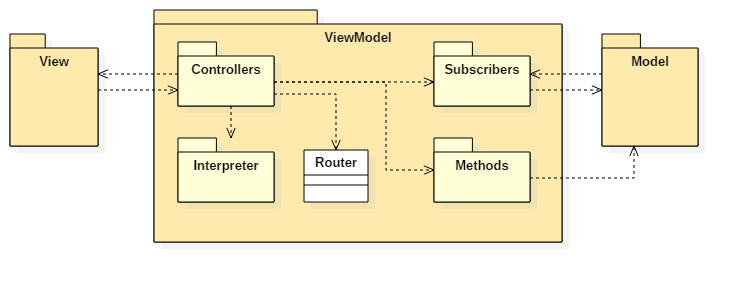
\includegraphics[scale=0.7]{../images/ViewModelPackage.png}
\end{center}
\end{figure}
\subsection{ViewModel::Controllers}
\subsubsection{ViewModel::Controllers::NewQuestionController}
\begin{itemize}
\item\textbf{Funzione del componente}: la classe permette di gestire la creazione di una nuova domanda
	\item\textbf{Relazione d'uso con altre componenti}: \\
La classe utilizza:
	\begin{itemize}
		\item QuestionMethods
		\item QuestionForm
	\end{itemize}
\item\textbf{Attributi}:
	\begin{itemize}
		\item\code{- \$scope}: Campo dati contenente un riferimento all’oggetto \$scope creato da Angular, viene utilizzato come mezzo di comunicazione tra il controller e il template.\\
	\end{itemize}
\item\textbf{Metodi}:
	\begin{itemize}
		\item\code{+ NewQuestionController()}: metodo costruttore della classe\\
		\textbf{Parametri}:
			\begin{itemize}
				\item\code{\$scope}: campo dati contenente un riferimento all’oggetto \$scope creato da Angular, viene utilizzato come mezzo di comunicazione tra il controller e il template.\\
			\end{itemize}
		\item\code{+ saveQuestion()}: metodo che permette il salvataggio di una nuova domanda tramite la chiamata ad un Method.\\
		\textbf{Parametri}:
			\begin{itemize}
				\item\code{question: String}: il testo QML della domanda da salvare.\\
				\item\code{category: String}: la categoria della domanda da salvare.\\
			\end{itemize}
	\end{itemize}
\end{itemize}

\subsubsection{ViewModel::Controllers::NewQuizController}
\begin{itemize}
\item\textbf{Funzione del componente}: la classe permette di gestire la creazione di un nuovo quiz (questionario);
\item\textbf{Relazioni con altre componenti}: \\
La classe utilizza:
	\begin{itemize}
		\item QuizMethods
		\item QuizCreationForm
	\end{itemize}
\item\textbf{Attributi}:
	\begin{itemize}
		\item\code{-\$scope}: Campo dati contenente un riferimento all'oggetto \$scope creato da Angular, viene utilizzato come mezzo di comunicazione tra il controller e il template.\\
	\end{itemize}
\item\textbf{Metodi}:
	\begin{itemize}
		\item\code{+ NewQuizController()}: metodo costruttore della classe\\
		\textbf{Parametri}:
			\begin{itemize}
				\item\code{\$scope}: campo dati contenente un riferimento all’oggetto \$scope creato da Angular, viene utilizzato come mezzo di comunicazione tra il controller e il template.\\
			\end{itemize}
		\item\code{+ saveQuiz()}\\
		\textbf{Parametri}:
			\begin{itemize}
				\item\code{title: String}: il titolo del questionario.\\
				\item\code{categories: Array}: la lista delle categorie associate al questionario.\\
				\item\code{questions: Array}: la lista di id delle domande che compongono il questionario.\\
				\item\code{time: Int}: il tempo massimo in minuti per la compilazione del questionario.\\
			\end{itemize}
	\end{itemize}
\end{itemize}

\subsubsection{ViewModel::Controllers::QuizListController}
\begin{itemize}
\item\textbf{Funzione del componente}:  la classe permette il caricamento e la visualizzazione della lista di quiz disponibili nel sistema
	\item\textbf{Relazione d'uso con altre componenti}:
La classe utilizza:
	\begin{itemize}
		\item QuizList
	\end{itemize}
\item\textbf{Attributi}:
	\begin{itemize}
		\item\code{\$scope}: Campo dati contenente un riferimento all’oggetto \$scope creato da Angular, viene utilizzato come mezzo di comunicazione tra il controller e il template.\\
	\end{itemize}
\item\textbf{Metodi}:
	\begin{itemize}
		\item\code{+ QuizListController()}: metodo costruttore della classe\\
		\textbf{Parametri}:
			\begin{itemize}
				\item\code{\$scope}: campo dati contenente un riferimento all’oggetto \$scope creato da Angular, viene utilizzato come mezzo di comunicazione tra il controller e il template.\\
			\end{itemize}
		\item\code{+ quizzes()}: metodo che ritorna la lista dei quiz del sistema.\\
		\item\code{+ quizDetails()}: metodo che permette la visualizzazione dei dettagli di un quiz.\\
		\textbf{Parametri}:
			\begin{itemize}
				\item\code{quizID: String}: identificativo univoco del quiz da visualizzare.\\
			\end{itemize}
		\item\code{+ orderBy()}: metodo che permette l'ordinamento della lista di quiz.\\
		\textbf{Parametri}:
			\begin{itemize}
				\item\code{orderBy: String}: il parametro in base al quale riordinare la lista di quiz.\\
			\end{itemize}
	\end{itemize}
\end{itemize}

\subsubsection{ViewModel::Controllers::QuizDetailsController}\begin{itemize}
\item\textbf{Funzione del componente}: la classe permette di visualizzare le informazioni generali di un quiz, una volta selezionato dalla lista dei quiz;
	\item\textbf{Relazione d'uso con altre componenti}: \\
La classe utilizza:
	\begin{itemize}
		\item
	\end{itemize}
\item\textbf{Attributi}:
	\begin{itemize}
		\item\code{- \$scope}: Campo dati contenente un riferimento all'oggetto \$scope creato da Angular, viene utilizzato come mezzo di comunicazione tra il controller e il template.\\
	\end{itemize}
\item\textbf{Metodi}:
	\begin{itemize}
		\item\code{+ QuizDetailsController()}: metodo costruttore della classe\\
		\textbf{Parametri}:
			\begin{itemize}
				\item\code{\$scope}: campo dati contenente un riferimento all’oggetto \$scope creato da Angular, viene utilizzato come mezzo di comunicazione tra il controller e il template.\\
			\end{itemize}
	\end{itemize}
\end{itemize}

\subsubsection{ViewModel::Controllers::DeleteQuestionController}
\begin{itemize}
\item\textbf{Funzione del componente}: la classe fornisce le funzionalità necessarie alla cancellazione di una domanda precedentemente creata;
	\item\textbf{Relazione d'uso con altre componenti}: \\
La classe utilizza:
	\begin{itemize}
		\item QuestionMethods
		\item QuestionList
	\end{itemize}
\item\textbf{Attributi}:
	\begin{itemize}
		\item\code{- \$scope}: Campo dati contenente un riferimento all’oggetto \$scope creato da Angular, viene utilizzato come mezzo di comunicazione tra il controller e il template.\\

	\end{itemize}
\item\textbf{Metodi}:
	\begin{itemize}
		\item\code{+ DeleteQuestionController()}: metodo costruttore della classe\\
		\textbf{Parametri}:
			\begin{itemize}
				\item\code{\$scope}: campo dati contenente un riferimento all’oggetto \$scope creato da Angular, viene utilizzato come mezzo di comunicazione tra il controller e il template.\\
			\end{itemize}
		\item\code{+ deleteQuestion()}\\
		\textbf{Parametri}:
			\begin{itemize}
				\item\code{question: String}: identificativo univoco della domanda da eliminare\\
			\end{itemize}
	\end{itemize}
\end{itemize}

\subsubsection{ViewModel::Controllers::DeleteQuizController}
\begin{itemize}
\item\textbf{Funzione del componente}: la classe fornisce le funzionalità necessarie alla cancellazione di un quiz precedentemente creato;
	\item\textbf{Relazione d'uso con altre componenti}: \\
La classe utilizza:
	\begin{itemize}
		\item QuizMethods
		\item QuizList
	\end{itemize}
\item\textbf{Attributi}:
	\begin{itemize}
		\item\code{- \$scope}: Campo dati contenente un riferimento all’oggetto \$scope creato da Angular, viene utilizzato come mezzo di comunicazione tra il controller e il template.\\
	\end{itemize}
\item\textbf{Metodi}:
	\begin{itemize}
		\item\code{+ DeleteQuizController()}: metodo costruttore della classe\\
		\textbf{Parametri}:
			\begin{itemize}
				\item\code{\$scope}: campo dati contenente un riferimento all’oggetto \$scope creato da Angular, viene utilizzato come mezzo di comunicazione tra il controller e il template.\\
			\end{itemize}
		\item\code{+ deleteQuiz()}\\
		\textbf{Parametri}:
			\begin{itemize}
				\item\code{quiz: String}: identificativo univoco del quiz da eliminare\\
			\end{itemize}
	\end{itemize}
\end{itemize}

\subsubsection{ViewModel::Controllers::QuizManagementController}
\begin{itemize}
\item\textbf{Funzione del componente}: la classe permette di gestire la somministrazione di un questionario;
	\item\textbf{Relazione d'uso con altre componenti}: \\
La classe utilizza:
	\begin{itemize}
		\item QuestionCompilation
	\end{itemize}
\item\textbf{Attributi}:
	\begin{itemize}
		\item\code{- \$scope}: Campo dati contenente un riferimento all’oggetto \$scope creato da Angular, viene utilizzato come mezzo di comunicazione tra il controller e il template.\\
	\end{itemize}
\item\textbf{Metodi}:
	\begin{itemize}
		\item\code{+QuizManagementController()}: metodo costruttore della classe\\
		\textbf{Parametri}:
			\begin{itemize}
				\item\code{\$scope}: campo dati contenente un riferimento all'oggetto \$scope creato da Angular, viene utilizzato come mezzo di comunicazione tra il controller e il template.\\
			\end{itemize}
		\item\code{+ nextQuestion()}: funzione che ritorna la domanda successiva nel questionario\\
		\textbf{Parametri}:
			\begin{itemize}
				\item\code{question: String}: identificativo univoco della domanda\\
			\end{itemize}
		\item\code{+ previousQuestion()}: funzione che ritorna la domanda precedente nel questionario\\
		\textbf{Parametri}:
			\begin{itemize}
				\item\code{question: String}: identificativo univoco della domanda\\
			\end{itemize}
		\item\code{+ endQuiz()}: metodo per la consegna del quiz in compilazione\\
	\end{itemize}
\end{itemize}

\subsubsection{ViewModel::Controllers::QuestionsManagementController}
\begin{itemize}
\item\textbf{Funzione del componente}: la classe permette di gestire la somministrazione di una singola domanda all'interno di un questionario;
	\item\textbf{Relazione d'uso con altre componenti}: \\
La classe utilizza:
	\begin{itemize}
		\item QuestionCompilation
		\item QuestionMethods
	\end{itemize}
\item\textbf{Attributi}:
	\begin{itemize}
		\item\code{- \$scope}: Campo dati contenente un riferimento all’oggetto \$scope creato da Angular, viene utilizzato come mezzo di comunicazione tra il controller e il template.\\
	\end{itemize}
\item\textbf{Metodi}:
	\begin{itemize}
		\item\code{+ QuestionsManagementController()}: metodo costruttore della classe\\
		\textbf{Parametri}:
			\begin{itemize}
				\item\code{\$scope}: campo dati contenente un riferimento all’oggetto \$scope creato da Angular, viene utilizzato come mezzo di comunicazione tra il controller e il template.\\
			\end{itemize}
		\item\code{+ getQuestion()}: metodo per caricare una domanda specifica\\
		\textbf{Parametri}:
			\begin{itemize}
				\item\code{question: String}: identificativo univoco della domanda\\
			\end{itemize}
	\end{itemize}
\end{itemize}

\subsubsection{ViewModel::Controllers::QMLEditorController}
\begin{itemize}
\item\textbf{Funzione del componente}: fornisce le funzionalità per creare e modificare una domanda tramite editor QML;
	\item\textbf{Relazione d'uso con altre componenti}: \\
La classe utilizza:
	\begin{itemize}
		\item NewQuestion
		\item QuestionMethods
	\end{itemize}
\item\textbf{Attributi}:
	\begin{itemize}
		\item\code{- \$scope}: Campo dati contenente un riferimento all’oggetto \$scope creato da Angular, viene utilizzato come mezzo di comunicazione tra il controller e il template.\\
	\end{itemize}
\item\textbf{Metodi}:
	\begin{itemize}
		\item\code{+ QMLEditorController()}: metodo costruttore della classe\\
		\textbf{Parametri}:
			\begin{itemize}
				\item\code{\$scope}: campo dati contenente un riferimento all’oggetto \$scope creato da Angular, viene utilizzato come mezzo di comunicazione tra il controller e il template.\\
			\end{itemize}
		\item\code{check()}: metodo che controlla che il testo QML inserito sia sintatticamente corretto\\
		\textbf{Parametri}:
			\begin{itemize}
				\item\code{text: String}: il testo QML inserito\\
			\end{itemize}
	\end{itemize}
\end{itemize}


\subsection{ViewModel::Subscribers}
\subsubsection{ViewModel::Subscribers::QuestionsSubscriber}
\begin{itemize}
\item\textbf{Funzione del componente}: la classe è necessaria ad effettuare il \emph{subscribe} relativo alla collezione di domande del sistema;
	\item\textbf{Relazione d'uso con altre componenti}: si relazione con la componente QuestionsManagementController;\\ \\
La classe utilizza:
	\begin{itemize}
		\item
	\end{itemize}
\item\textbf{Attributi}:
	\begin{itemize}
		\item\code{}\\
		\item\code{}\\
		\item\code{}\\
		\item\code{}\\
	\end{itemize}
\item\textbf{Metodi}:
	\begin{itemize}
		\item\code{}\\
		\textbf{Parametri}:
			\begin{itemize}
				\item\code{}\\
			\end{itemize}
		\item\code{}\\
		\textbf{Parametri}:
			\begin{itemize}
				\item\code{}\\
			\end{itemize}
		\item\code{}\\
		\textbf{Parametri}:
			\begin{itemize}
				\item\code{}\\
			\end{itemize}
		\item\code{}\\
		\textbf{Parametri}:
			\begin{itemize}
				\item\code{}\\
			\end{itemize}
	\end{itemize}
\end{itemize}

\subsubsection{ViewModel::Subscribers::QuizSubscriber}
\begin{itemize}
\item\textbf{Funzione del componente}: la classe è necessaria ad effettuare il \emph{subscribe} relativo alla collezione di quiz del sistema;
	\item\textbf{Relazione d'uso con altre componenti}: si relazione con le componenti QuizListController e QuizManagementController;\\ \\
La classe utilizza:
	\begin{itemize}
		\item
	\end{itemize}
\item\textbf{Attributi}:
	\begin{itemize}
		\item\code{}\\
		\item\code{}\\
		\item\code{}\\
		\item\code{}\\
	\end{itemize}
\item\textbf{Metodi}:
	\begin{itemize}
		\item\code{}\\
		\textbf{Parametri}:
			\begin{itemize}
				\item\code{}\\
			\end{itemize}
		\item\code{}\\
		\textbf{Parametri}:
			\begin{itemize}
				\item\code{}\\
			\end{itemize}
		\item\code{}\\
		\textbf{Parametri}:
			\begin{itemize}
				\item\code{}\\
			\end{itemize}
		\item\code{}\\
		\textbf{Parametri}:
			\begin{itemize}
				\item\code{}\\
			\end{itemize}
	\end{itemize}
\end{itemize}

\subsubsection{ViewModel::Subscribers::UsersSubscriber}
\begin{itemize}
\item\textbf{Funzione del componente}: la classe è necessaria ad effettuare il \emph{subscribe} relativo alla collezione di utenti del sistema;
	\item\textbf{Relazione d'uso con altre componenti}: si relaziona con il package esterno 'accounts-ui';\\ 
La classe utilizza:
	\begin{itemize}
		\item
	\end{itemize}
\item\textbf{Attributi}:
	\begin{itemize}
		\item\code{}\\
		\item\code{}\\
		\item\code{}\\
		\item\code{}\\
	\end{itemize}
\item\textbf{Metodi}:
	\begin{itemize}
		\item\code{}\\
		\textbf{Parametri}:
			\begin{itemize}
				\item\code{}\\
			\end{itemize}
		\item\code{}\\
		\textbf{Parametri}:
			\begin{itemize}
				\item\code{}\\
			\end{itemize}
		\item\code{}\\
		\textbf{Parametri}:
			\begin{itemize}
				\item\code{}\\
			\end{itemize}
		\item\code{}\\
		\textbf{Parametri}:
			\begin{itemize}
				\item\code{}\\
			\end{itemize}
	\end{itemize}
\end{itemize}

\subsection{ViewModel::Methods}
\subsubsection{ViewModel::Methods::QuestionMethods}
\begin{itemize}
\item\textbf{Funzione del componente}: permette al client di richiedere la modifica della collezione di domande del server;
	\item\textbf{Relazione d'uso con altre componenti}: si relaziona con le classi NewQuestionController e DeleteQuestionController;\\ \\
La classe utilizza:
	\begin{itemize}
		\item
	\end{itemize}
\item\textbf{Attributi}:
	\begin{itemize}
		\item\code{}\\
		\item\code{}\\
		\item\code{}\\
		\item\code{}\\
	\end{itemize}
\item\textbf{Metodi}:
	\begin{itemize}
		\item\code{}\\
		\textbf{Parametri}:
			\begin{itemize}
				\item\code{}\\
			\end{itemize}
		\item\code{}\\
		\textbf{Parametri}:
			\begin{itemize}
				\item\code{}\\
			\end{itemize}
		\item\code{}\\
		\textbf{Parametri}:
			\begin{itemize}
				\item\code{}\\
			\end{itemize}
		\item\code{}\\
		\textbf{Parametri}:
			\begin{itemize}
				\item\code{}\\
			\end{itemize}
	\end{itemize}
\end{itemize}

\subsubsection{ViewModel::Methods::QuizMethods}
\begin{itemize}
\item\textbf{Funzione del componente}: permette al client di richiedere la modifica della collezione di quiz del server;
	\item\textbf{Relazione d'uso con altre componenti}: si relaziona con le classi NewQuizController e DeleteQuizController;\\ \\
La classe utilizza:
	\begin{itemize}
		\item
	\end{itemize}
\item\textbf{Attributi}:
	\begin{itemize}
		\item\code{}\\
		\item\code{}\\
		\item\code{}\\
		\item\code{}\\
	\end{itemize}
\item\textbf{Metodi}:
	\begin{itemize}
		\item\code{}\\
		\textbf{Parametri}:
			\begin{itemize}
				\item\code{}\\
			\end{itemize}
		\item\code{}\\
		\textbf{Parametri}:
			\begin{itemize}
				\item\code{}\\
			\end{itemize}
		\item\code{}\\
		\textbf{Parametri}:
			\begin{itemize}
				\item\code{}\\
			\end{itemize}
		\item\code{}\\
		\textbf{Parametri}:
			\begin{itemize}
				\item\code{}\\
			\end{itemize}
	\end{itemize}
\end{itemize}

\subsubsection{ViewModel::Methods::UserMethods}
\begin{itemize}
\item\textbf{Funzione del componente}: permette al client di richiedere la modifica della collezione di utenti del server;
	\item\textbf{Relazione d'uso con altre componenti}:  si relaziona con il package esterno 'accounts-ui';\\ \\
La classe utilizza:
	\begin{itemize}
		\item
	\end{itemize}
\item\textbf{Attributi}:
	\begin{itemize}
		\item\code{}\\
		\item\code{}\\
		\item\code{}\\
		\item\code{}\\
	\end{itemize}
\item\textbf{Metodi}:
	\begin{itemize}
		\item\code{}\\
		\textbf{Parametri}:
			\begin{itemize}
				\item\code{}\\
			\end{itemize}
		\item\code{}\\
		\textbf{Parametri}:
			\begin{itemize}
				\item\code{}\\
			\end{itemize}
		\item\code{}\\
		\textbf{Parametri}:
			\begin{itemize}
				\item\code{}\\
			\end{itemize}
		\item\code{}\\
		\textbf{Parametri}:
			\begin{itemize}
				\item\code{}\\
			\end{itemize}
	\end{itemize}
\end{itemize}

\subsection{ViewModel::Interpreter}
\subsubsection{ViewModel::Interpreter::Interpreter}
\begin{itemize}
\item\textbf{Funzione del componente}: interfaccia di base del tipo Interpreter.
	\item\textbf{Relazione d'uso con altre componenti}: può essere concretizzata in diversi tipi di Interpreter.\\ \\
La classe utilizza:
	\begin{itemize}
		\item
	\end{itemize}
\item\textbf{Attributi}:
	\begin{itemize}
		\item\code{}\\
		\item\code{}\\
		\item\code{}\\
		\item\code{}\\
	\end{itemize}
\item\textbf{Metodi}:
	\begin{itemize}
		\item\code{}\\
		\textbf{Parametri}:
			\begin{itemize}
				\item\code{}\\
			\end{itemize}
		\item\code{}\\
		\textbf{Parametri}:
			\begin{itemize}
				\item\code{}\\
			\end{itemize}
		\item\code{}\\
		\textbf{Parametri}:
			\begin{itemize}
				\item\code{}\\
			\end{itemize}
		\item\code{}\\
		\textbf{Parametri}:
			\begin{itemize}
				\item\code{}\\
			\end{itemize}
	\end{itemize}
\end{itemize}

\subsubsection{ViewModel::Interpreter::InterpreterFactory}
\begin{itemize}
\item\textbf{Funzione del componente}: interfaccia di base delle Factory di tipi Interpreter.
	\item\textbf{Relazione d'uso con altre componenti}: può essere concretizzata in diversi tipi di InterpreterFactory.\\ \\
La classe utilizza:
	\begin{itemize}
		\item
	\end{itemize}
\item\textbf{Attributi}:
	\begin{itemize}
		\item\code{}\\
		\item\code{}\\
		\item\code{}\\
		\item\code{}\\
	\end{itemize}
\item\textbf{Metodi}:
	\begin{itemize}
		\item\code{}\\
		\textbf{Parametri}:
			\begin{itemize}
				\item\code{}\\
			\end{itemize}
		\item\code{}\\
		\textbf{Parametri}:
			\begin{itemize}
				\item\code{}\\
			\end{itemize}
		\item\code{}\\
		\textbf{Parametri}:
			\begin{itemize}
				\item\code{}\\
			\end{itemize}
		\item\code{}\\
		\textbf{Parametri}:
			\begin{itemize}
				\item\code{}\\
			\end{itemize}
	\end{itemize}
\end{itemize}

\subsubsection{ViewModel::Interpreter::QMLInterpreterFactory}
\begin{itemize}
\item\textbf{Funzione del componente}: crea oggetti di tipo QMLInterpreter.
	\item\textbf{Relazione d'uso con altre componenti}: è concretizzazione della classe InterpreterFactory. Crea oggetti QMLInterpreter.\\ \\
La classe utilizza:
	\begin{itemize}
		\item
	\end{itemize}
\item\textbf{Attributi}:
	\begin{itemize}
		\item\code{}\\
		\item\code{}\\
		\item\code{}\\
		\item\code{}\\
	\end{itemize}
\item\textbf{Metodi}:
	\begin{itemize}
		\item\code{}\\
		\textbf{Parametri}:
			\begin{itemize}
				\item\code{}\\
			\end{itemize}
		\item\code{}\\
		\textbf{Parametri}:
			\begin{itemize}
				\item\code{}\\
			\end{itemize}
		\item\code{}\\
		\textbf{Parametri}:
			\begin{itemize}
				\item\code{}\\
			\end{itemize}
		\item\code{}\\
		\textbf{Parametri}:
			\begin{itemize}
				\item\code{}\\
			\end{itemize}
	\end{itemize}
\end{itemize}

\subsubsection{ViewModel::Interpreter::QMLInterpreter}
\begin{itemize}
\item\textbf{Funzione del componente}: classe astratta che rappresenta gli Interpreter che traducono codice QML in un altro formato.
	\item\textbf{Relazione d'uso con altre componenti}: è sottotipo di Interpreter. Può essere concretizzata in più tipi di QMLInterpreter.\\ \\
La classe utilizza:
	\begin{itemize}
		\item
	\end{itemize}
\item\textbf{Attributi}:
	\begin{itemize}
		\item\code{}\\
		\item\code{}\\
		\item\code{}\\
		\item\code{}\\
	\end{itemize}
\item\textbf{Metodi}:
	\begin{itemize}
		\item\code{}\\
		\textbf{Parametri}:
			\begin{itemize}
				\item\code{}\\
			\end{itemize}
		\item\code{}\\
		\textbf{Parametri}:
			\begin{itemize}
				\item\code{}\\
			\end{itemize}
		\item\code{}\\
		\textbf{Parametri}:
			\begin{itemize}
				\item\code{}\\
			\end{itemize}
		\item\code{}\\
		\textbf{Parametri}:
			\begin{itemize}
				\item\code{}\\
			\end{itemize}
	\end{itemize}
\end{itemize}

\subsubsection{ViewModel::Interpreter::QML2HTMLInterpreterFactory}
\begin{itemize}
\item\textbf{Funzione del componente}: traduce codice QML in codice HTML.
	\item\textbf{Relazione d'uso con altre componenti}: è concretizzazione di QMLInterpreter.\\ \\
La classe utilizza:
	\begin{itemize}
		\item
	\end{itemize}
\item\textbf{Attributi}:
	\begin{itemize}
		\item\code{}\\
		\item\code{}\\
		\item\code{}\\
		\item\code{}\\
	\end{itemize}
\item\textbf{Metodi}:
	\begin{itemize}
		\item\code{}\\
		\textbf{Parametri}:
			\begin{itemize}
				\item\code{}\\
			\end{itemize}
		\item\code{}\\
		\textbf{Parametri}:
			\begin{itemize}
				\item\code{}\\
			\end{itemize}
		\item\code{}\\
		\textbf{Parametri}:
			\begin{itemize}
				\item\code{}\\
			\end{itemize}
		\item\code{}\\
		\textbf{Parametri}:
			\begin{itemize}
				\item\code{}\\
			\end{itemize}
	\end{itemize}
\end{itemize}


\subsection{ViewModel::Router}
\subsubsection{ViewModel::Router::Router}
\begin{itemize}
\item\textbf{Funzione del componente}: implementa il routing dinamico dell'applicazione. Permette di dividere la parte statica dell'applicazione dalla parte che va caricata dinamicamente;
	\item\textbf{Relazione d'uso con altre componenti}: Utilizza il package esterno ui-router. Conosce i Template dell'applicazione.\\ \\
La classe utilizza:
	\begin{itemize}
		\item
	\end{itemize}
\item\textbf{Attributi}:
	\begin{itemize}
		\item\code{}\\
		\item\code{}\\
		\item\code{}\\
		\item\code{}\\
	\end{itemize}
\item\textbf{Metodi}:
	\begin{itemize}
		\item\code{}\\
		\textbf{Parametri}:
			\begin{itemize}
				\item\code{}\\
			\end{itemize}
		\item\code{}\\
		\textbf{Parametri}:
			\begin{itemize}
				\item\code{}\\
			\end{itemize}
		\item\code{}\\
		\textbf{Parametri}:
			\begin{itemize}
				\item\code{}\\
			\end{itemize}
		\item\code{}\\
		\textbf{Parametri}:
			\begin{itemize}
				\item\code{}\\
			\end{itemize}
	\end{itemize}
\end{itemize}